%%%%%%%%%%%%%%%%%%%%%%%%%%%%%%%%%%%%%%%%%%%%%%%%%%%%%%%%%%%%%%%%%%%%%%
% Skupina08/main.tex
% Primerjava kvantnih seštevalnikov CDKM in Draper na procesorjih IBM
%%%%%%%%%%%%%%%%%%%%%%%%%%%%%%%%%%%%%%%%%%%%%%%%%%%%%%%%%%%%%%%%%%%%%%

\graphicspath{{Skupina08/img/}}

\title{Primerjava kvantnih seštevalnikov CDKM in Draper (QFT) na šumnem kvantnem procesorju IBM}
\toctitle{Primerjava kvantnih seštevalnikov CDKM in Draper (QFT)\newline na šumnem kvantnem procesorju IBM}
\titlerunning{Seštevalnika CDKM in Draper na procesorju IBM}
\author{Jurij Anžič in Janez Koprivec}
\maketitle

\abstract{Primerjala sva kvantni seštevalnik CDKM z zaporednim prenosom (linearno število vrat) in Draperjev seštevalnik na osnovi kvantne Fourierjeve transformacije (kvadratno število vrat). Zanimalo naju je, kateri na procesorju IBM pogosteje vrne pravilno vsoto in ali to napove število dvokubitnih vrat po prevajanju. Seštevalnika sva izvedla na simulatorjih ter na procesorjih ibm\_fez in ibm\_kingston, z dinamičnim razklapljanjem (DD) in brez njega. CDKM ima od $n = 4$ naprej manj dvokubitnih vrat, vendar brez DD to v 8 od 9 primerjav ni napovedalo boljšega seštevalnika. Z DD je napoved veljala v vseh 7 primerjavah: pri $n = 8$ je CDKM vrnil pravilno vsoto v 21~\% ponovitev, Draper v 8~\%. Število dvokubitnih vrat je torej dober napovedovalec šele, ko so zadušene napake med mirovanjem kubitov.}


\section{Uvod}
\label{g08:sec:uvod}

Kvantni algoritmi, ki obljubljajo pohitritev, pogosto potrebujejo aritmetiko na kvantnih registrih. Najbolj znan primer je Shorov algoritem~\cite{shor1997}, katerega najzahtevnejši del je modularno potenciranje, sestavljeno iz množenj, ta pa iz seštevanj~\cite{g08:vedral1996}. Seštevalnik je zato osnovni gradnik kvantne aritmetike in hkrati priročno merilo zmogljivosti kvantnih procesorjev: pravilen rezultat je znan vnaprej in je en sam izid, zato je uspešnost preprosto izmeriti~\cite{g08:nishio2020}.

Kvantni seštevalniki se delijo na dve družini. Prva prenaša klasično reverzibilno logiko na kubite. Vedral, Barenco in Ekert~\cite{g08:vedral1996} so predstavili seštevalnik z zaporednim prenosom (angl.\ ripple-carry), ki potrebuje linearno mnogo pomožnih kubitov. Cuccaro, Draper, Kutin in Moulton (CDKM)~\cite{g08:cuccaro2004} so ga izboljšali tako, da potrebuje en sam pomožni kubit ter ima manj vrat in manjšo globino. Druga družina izkorišča kvantne lastnosti: Draper~\cite{g08:draper2000} je pokazal, da lahko seštevamo v Fourierjevi bazi, kjer je prištevanje števila le zasuk faz. Tak seštevalnik ne potrebuje nobenega pomožnega kubita, ima pa kvadratno mnogo kontroliranih faznih vrat.

Današnji kvantni procesorji so šumni in imajo omejeno povezljivost kubitov~\cite{preskill2018}. Pri prevajanju (angl.\ transpilation) se vezje razgradi na vrata, ki jih procesor izvaja neposredno, in dobi vrata SWAP med nepovezanimi kubiti. Ker so dvokubitna vrata največji vir napak, se pogosto privzame, da je vezje z manj dvokubitnimi vrati uspešnejše. Nishio in sod.~\cite{g08:nishio2020} so pokazali, da je ocena uspešnosti iz napak posameznih vrat uporabno, a nepopolno vodilo. Na uspešnost vpliva tudi čas, ko kubiti čakajo na druge kubite. Med mirovanjem izgubljajo koherenco in so izpostavljeni presluhu sosednjih kubitov, kar lahko delno odpravi dinamično razklapljanje (angl.\ dynamical decoupling, DD)~\cite{g08:viola1999,g08:tripathi2022,g08:ezzell2023}. Basili in sod.~\cite{g08:basili2025} so seštevalnike na osnovi QFT ovrednotili s šumnimi modeli, neposredne primerjave obeh družin na sodobnem procesorju z enakimi nastavitvami pa nisva našla.

\begin{svgraybox}
\textbf{Raziskovalno vprašanje.} Kateri seštevalnik, CDKM ali Draper, na procesorju IBM pogosteje vrne pravilno vsoto in ali to napove število dvokubitnih vrat po prevajanju?

\textbf{Pričakovani rezultat.} Pri vsakem $n$ od $2$ do $5$ bo CDKM na procesorju IBM imel višjo verjetnost pravilne vsote kot Draper, ker bo imel po prevajanju manj dvokubitnih vrat.
\end{svgraybox}

V razdelku~\ref{g08:sec:metode} opiševa oba seštevalnika, orodja in poskuse. V razdelku~\ref{g08:sec:rezultati} predstaviva lastnosti vezij in uspešnost na simulatorjih in procesorjih, v razdelku~\ref{g08:sec:razprava} pa odgovoriva na raziskovalno vprašanje in opiševa, kaj ni delovalo.


\section{Metode}
\label{g08:sec:metode}

\subsection{Seštevalnika}
\label{g08:sec:sestevalnika}

Oba seštevalnika izvedeta preslikavo $\ket{a}\ket{b} \mapsto \ket{a}\ket{a+b}$. Register $a$ ima $n$ kubitov, register $b$ pa $n+1$: zgornji kubit je na začetku $0$ in na koncu vsebuje izhodni prenos, zato je vsota točna. Obe implementaciji vrneta samo seštevalnik, brez priprave vhodov in meritev, tako da vhodi ne vplivajo na lastnosti vezja.

\smallskip\noindent\textbf{CDKM.} Seštevalnik je sestavljen iz dveh vrst blokov na treh kubitih (slika~\ref{g08:fig:majuma}). Blok MAJ izračuna prenos $c_{i+1} = \mathrm{MAJ}(a_i, b_i, c_i)$ in ga zapiše na mesto $a_i$, zato prenos ne potrebuje svojih kubitov. Veriga blokov MAJ gre od najnižjega bita navzgor, vrata CNOT prepišejo zgornji prenos v $b_n$, veriga blokov UMA pa gre nazaj navzdol: vsak blok razveljavi svoj MAJ, vrne $a_i$ v prvotno stanje in v $b_i$ zapiše bit vsote $s_i = a_i \oplus b_i \oplus c_i$ (slika~\ref{g08:fig:cdkm}). Vezje ima $2n+2$ kubitov (en pomožni za $c_0 = 0$), $2n$ Toffolijevih vrat in $4n+1$ vrat CNOT. Ker so vsi bloki zaporedni, je globina linearna v $n$.

\begin{figure}[tbp]
\centering
\begin{subfigure}[b]{0.42\textwidth}
\centering
\small
\begin{quantikz}[row sep=0.2cm, column sep=0.15cm]
\lstick{$c$} & & \targ{} & \ctrl{2} & \rstick{$c \oplus a$} \\
\lstick{$b$} & \targ{} & & \ctrl{1} & \rstick{$b \oplus a$} \\
\lstick{$a$} & \ctrl{-1} & \ctrl{-2} & \targ{} & \rstick{$\mathrm{MAJ}(a,b,c)$}
\end{quantikz}\\[0.3cm]
\begin{quantikz}[row sep=0.2cm, column sep=0.15cm]
\lstick{$c \oplus a$} & \ctrl{2} & \targ{} & \ctrl{1} & \rstick{$c$} \\
\lstick{$b \oplus a$} & \ctrl{1} & & \targ{} & \rstick{$s$} \\
\lstick{$\mathrm{MAJ}$} & \targ{} & \ctrl{-2} & & \rstick{$a$}
\end{quantikz}
\caption{bloka MAJ (zgoraj) in UMA (spodaj)}
\label{g08:fig:majuma}
\end{subfigure}
\hfill
\begin{subfigure}[b]{0.54\textwidth}
\centering
\small
\scalebox{0.88}{\begin{quantikz}[row sep=0.15cm, column sep=0.2cm]
\lstick{$c_0 = 0$} & \gate[3]{\mathrm{MAJ}} & & & & \gate[3]{\mathrm{UMA}} & \rstick{$0$} \\
\lstick{$b_0$} & & & & & & \rstick{$s_0$} \\
\lstick{$a_0$} & & \gate[3]{\mathrm{MAJ}} & & \gate[3]{\mathrm{UMA}} & & \rstick{$a_0$} \\
\lstick{$b_1$} & & & & & & \rstick{$s_1$} \\
\lstick{$a_1$} & & & \ctrl{1} & & & \rstick{$a_1$} \\
\lstick{$b_2 = 0$} & & & \targ{} & & & \rstick{$s_2$}
\end{quantikz}}
\caption{seštevalnik za $n = 2$}
\label{g08:fig:cdkm}
\end{subfigure}
\caption{Seštevalnik CDKM~\cite{g08:cuccaro2004}. Bloka MAJ in UMA delujeta na treh kubitih, $s = a \oplus b \oplus c$. Prenos potuje navzgor po verigi blokov MAJ in se vrača navzdol po verigi blokov UMA.}
\label{g08:fig:cdkmvse}
\end{figure}

\smallskip\noindent\textbf{Draper.} Kvantna Fourierjeva transformacija (QFT)~\cite{nielsen2010} na registru $b$ z $m = n+1$ kubiti zapiše število $b$ v faze posameznih kubitov:
\begin{equation}
\mathrm{QFT}\ket{b} = \bigotimes_{k=0}^{m-1} \frac{\ket{0} + e^{2\pi i\, b / 2^{k+1}} \ket{1}}{\sqrt{2}} .
\label{g08:eq:qft}
\end{equation}
Prištevanje $a$ je v tej bazi zasuk faze kubita $k$ za $2\pi a / 2^{k+1} = \sum_j a_j\, \pi / 2^{k-j}$. Vsak člen izvedejo kontrolirana fazna vrata $P(\pi/2^{k-j})$, ki jih krmili bit $a_j$; člene z $j > k$ izpustimo, ker je njihov kot večkratnik $2\pi$. Inverzna QFT nato vrne $b$ v računsko bazo, kjer je zapisana vsota (slika~\ref{g08:fig:draper}). Vezje nima pomožnih kubitov, ima pa $\tfrac{3}{2}n(n+1) + n$ kontroliranih faznih vrat, torej kvadratno mnogo. Uporabila sva točno QFT brez končnih vrat SWAP, ki bi se pri QFT in inverzni QFT izničila.

\begin{figure}[tbp]
\centering
\begin{quantikz}[row sep=0.25cm, column sep=0.25cm]
\lstick{$a_0$} & & & & \ctrl{1} & \ctrl{2} & & & & \rstick{$a_0$} \\
\lstick{$b_0$} & \gategroup[2,steps=3,style={dashed,rounded corners,inner xsep=2pt},label style={label position=below,anchor=north,yshift=-0.2cm}]{QFT} & \ctrl{1} & \gate{H} & \gate{P(\pi)} & & \gate{H} \gategroup[2,steps=3,style={dashed,rounded corners,inner xsep=2pt},label style={label position=below,anchor=north,yshift=-0.2cm}]{QFT$^{-1}$} & \ctrl{1} & & \rstick{$s_0$} \\
\lstick{$b_1 = 0$} & \gate{H} & \gate{P(\frac{\pi}{2})} & & & \gate{P(\frac{\pi}{2})} & & \gate{P(-\frac{\pi}{2})} & \gate{H} & \rstick{$s_1$}
\end{quantikz}
\vspace{0.4cm}
\caption{Draperjev seštevalnik za $n = 1$. Med QFT in inverzno QFT bit $a_0$ krmili dvoje faznih vrat, ki prištejejo $a_0$ v Fourierjevi bazi.}
\label{g08:fig:draper}
\end{figure}

\subsection{Orodja in nastavitve}
\label{g08:sec:orodja}

Vezja sva napisala v Qiskitu~\cite{qiskit2024}, simulirala s Qiskit Aer~\cite{g08:qiskitaer} in poslala na procesorje IBM prek storitve Qiskit Runtime (Sampler V2) v brezplačnem paketu Open Plan (600~s procesorskega časa na 28 dni). Nastavitve so v tabeli~\ref{g08:tab:nastavitve}. Datoteka README v repozitoriju opisuje, kako ponovimo vse rezultate; na simulatorjih so ponovljivi bit za bitom.

\begin{table}[tbp]
\caption{Orodja in nastavitve. Enake so za oba seštevalnika.}
\label{g08:tab:nastavitve}
\centering
\small
\begin{tabular}{ll}
\toprule
Nastavitev & Vrednost \\
\midrule
Python, Qiskit, Qiskit Aer & 3.12, 2.6.2, 0.18.4 \\
qiskit-ibm-runtime & 0.52.1 (šumni modeli FakeTorino, FakeFez) \\
procesorja & ibm\_fez, ibm\_kingston (IBM Heron r2, 156 kubitov) \\
osnovna vrata procesorja & CZ, $\sqrt{X}$, $X$, $R_Z$ \\
prevajanje & \texttt{optimization\_level=3}, \texttt{seed\_transpiler=2026} \\
ponovitve (angl.\ shots) & 1000 na vezje \\
seme šumnega simulatorja & \texttt{seed\_simulator=2026} \\
blaženje napak & brez (twirling izklopljen) \\
dinamično razklapljanje & izklopljeno ali zaporedje XpXm \\
\bottomrule
\end{tabular}
\end{table}

\subsection{Zasnova poskusov}
\label{g08:sec:poskusi}

Za vsak $n$ sva za oba seštevalnika uporabila iste pare vhodov: vse pare pri $n \le 2$ in 16 različnih naključnih parov pri $n \ge 3$, izbranih s fiksnim semenom. Vsako vezje sestavljajo vrata $X$ za pripravo vhodov, seštevalnik in meritev registra $b$. Pravilnost obeh seštevalnikov sva za vse pare vhodov pri $n = 1$ do $5$ preverila na idealnem simulatorju stanja (testi \texttt{pytest}). Nato sva vezja prevedla za šumna modela FakeTorino in FakeFez, zapisala njihove lastnosti pri šestih semenih prevajalnika in jih izvedla na idealnem in šumnem simulatorju.

Na procesorja IBM sva poslala sedem opravil (tabela~\ref{g08:tab:opravila}). Vsa vezja enega poskusa so v enem opravilu, zato oba seštevalnika vidita enako kalibracijo. Porabo celotnega opravila sva ocenila iz majhnega poskusnega opravila ($n = 1$). Na ibm\_fez sva opravilo brez DD ponovila, da sva ocenila razlike med zagoni, na ibm\_kingston pa sva poskus razširila na $n = 8$.

\begin{table}[tbp]
\caption{Opravila na procesorjih IBM (21.~11.~2026, čas UTC). Vsa imajo 1000 ponovitev na vezje.}
\label{g08:tab:opravila}
\centering
\small
\begin{tabular}{llcclrr}
\toprule
Procesor & $n$ & DD & Vezij & Job ID & Oddano & Poraba \\
\midrule
ibm\_fez & 1 & ne & 8 & \texttt{dc0r00ls2omc7389ndn0} & 14:51 & 4~s \\
ibm\_fez & 1--5 & ne & 136 & \texttt{dc0rbg5hdvas73bjutd0} & 15:16 & 39~s \\
ibm\_fez & 1--5 & da & 136 & \texttt{dc0rgfmq4uuc73a32e8g} & 15:26 & 39~s \\
ibm\_fez & 1--5 & ne & 136 & \texttt{dc0rh8ls2omc7389oddg} & 15:28 & 39~s \\
ibm\_kingston & 1 & ne & 8 & \texttt{dc0rifmq4uuc73a32hp0} & 15:31 & 4~s \\
ibm\_kingston & 1--8 & ne & 232 & \texttt{dc0riplhdvas73bjvamg} & 15:31 & 66~s \\
ibm\_kingston & 1--8 & da & 232 & \texttt{dc0rjn2nj2vs73defojg} & 15:33 & 66~s \\
\bottomrule
\end{tabular}
\end{table}

\subsection{Metrike}
\label{g08:sec:metrike}

\smallskip\noindent\textbf{Verjetnost pravilne vsote.} Za vsako vezje je to delež ponovitev, pri katerih je izmerjeni register $b$ enak $a+b$. Povprečimo jo po vseh parih vhodov pri danem $n$ in primerjamo z verjetnostjo naključnega izida $1/2^{n+1}$. Pri 1000 ponovitvah in 16 parih je statistična napaka povprečja zaradi končnega števila ponovitev okoli 0,004, razlike med zagonoma istega opravila pa so do 0,03 (razdelek~\ref{g08:sec:procesor}).

\smallskip\noindent\textbf{Lastnosti vezja.} Število kubitov, globino in število dvokubitnih vrat merimo na samem seštevalniku pred prevajanjem in po njem. Ker ima CDKM pred prevajanjem trokubitna Toffolijeva vrata, štejemo še vrata CNOT po razgradnji brez topologije procesorja (Toffolijeva vrata stanejo 6 CNOT, kontrolirana fazna 2).

\smallskip\noindent\textbf{Ocena uspešnosti iz kalibracije.} Za vsako opravilo IBM sva prenesla dejansko izvedena vezja (s fizičnimi kubiti) in kalibracijo procesorja v času izvajanja. Ocena verjetnosti uspeha (angl.\ estimated success probability, ESP)~\cite{g08:nishio2020} je
\begin{equation}
\mathrm{ESP} = \prod_{g} (1 - \varepsilon_g),
\label{g08:eq:esp}
\end{equation}
kjer produkt teče po vseh vratih in meritvah vezja, $\varepsilon_g$ pa je napaka vrat $g$ na dejanskih fizičnih kubitih iz kalibracije. ESP ne upošteva mirovanja, presluha in koherentnih napak, zato sva iz trajanja vrat izračunala še čas izvajanja vezja in skupni čas mirovanja kubitov. Kako dobro posamezna količina napove uspešnost, merimo s Pearsonovim korelacijskim koeficientom $r$ na vseh vezjih opravila. Za vsako opravilo in $n$ preverimo še, ali ima seštevalnik z manj dvokubitnimi vrati tudi višjo povprečno uspešnost.


\section{Rezultati}
\label{g08:sec:rezultati}

\subsection{Lastnosti vezij}
\label{g08:sec:lastnosti}

Tabela~\ref{g08:tab:lastnosti} kaže lastnosti vezij. Pred prevajanjem je število vrat CNOT po razgradnji pri CDKM enako $16n+1$, pri Draperju pa $3n(n+1)+2n$. Pri $n \le 3$ ima manj vrat Draper, pri $n = 4$ sta skoraj enaka, pri $n = 5$ ima CDKM 81 vrat CNOT, Draper pa 100. Prevajanje za procesor Heron obe vezji podaljša, Draperjevo pa bistveno bolj: fazna vrata povezujejo vsak kubit registra $b$ z vsemi drugimi, procesor pa ima vsak kubit povezan z največ tremi sosedi, zato prevajalnik doda veliko vrat SWAP. Po prevajanju ima CDKM manj dvokubitnih vrat od $n = 4$ naprej, pri $n = 3$ sta enaka (70), pri $n \le 2$ pa ima manj vrat Draper.

\begin{table}[tbp]
\caption{Lastnosti seštevalnikov pred prevajanjem in po njem za FakeFez (na ibm\_fez in ibm\_kingston je število dvokubitnih vrat enako). V oklepaju je razpon pri šestih semenih prevajalnika. Globina pred prevajanjem šteje Toffolijeva vrata kot en korak, zato med seštevalnikoma ni primerljiva.}
\label{g08:tab:lastnosti}
\centering
\small
\setlength{\tabcolsep}{4pt}
\begin{tabular}{rlrrrrrr}
\toprule
 & & & \multicolumn{3}{c}{pred prevajanjem} & \multicolumn{2}{c}{po prevajanju} \\
\cmidrule(lr){4-6}\cmidrule(lr){7-8}
$n$ & Seštevalnik & Kubiti & Globina & 2q / 3q & CNOT razgr. & 2q & Globina \\
\midrule
1 & CDKM & 4 & 7 & 5 / 2 & 17 & 22 (22--22) & 73 \\
  & Draper & 3 & 7 & 4 / 0 & 8 & 10 (10--10) & 39 \\
2 & CDKM & 6 & 12 & 9 / 4 & 33 & 46 (43--48) & 147 \\
  & Draper & 5 & 12 & 11 / 0 & 22 & 29 (29--33) & 96 \\
3 & CDKM & 8 & 17 & 13 / 6 & 49 & 70 (67--72) & 217 \\
  & Draper & 7 & 17 & 21 / 0 & 42 & 70 (68--82) & 188 \\
4 & CDKM & 10 & 22 & 17 / 8 & 65 & 94 (94--94) & 286 \\
  & Draper & 9 & 22 & 34 / 0 & 68 & 139 (121--144) & 265 \\
5 & CDKM & 12 & 27 & 21 / 10 & 81 & 124 (124--130) & 371 \\
  & Draper & 11 & 27 & 50 / 0 & 100 & 195 (177--211) & 374 \\
\bottomrule
\end{tabular}
\end{table}

\subsection{Simulatorji}
\label{g08:sec:simulatorji}

Na idealnem simulatorju sta oba seštevalnika za vse pare vhodov vrnila pravilno vsoto. Na šumnem simulatorju z modelom FakeFez je bil Draper boljši pri $n \le 2$, pri $n = 3$ sta bila izenačena (0,80), pri $n = 4$ in $5$ pa je bil boljši CDKM (pri $n = 5$ 0,69 proti 0,54). Model FakeTorino je dal podoben vzorec. Šumni simulator je torej napovedal, da bo CDKM boljši od $n = 3$ ali $4$ naprej.

\subsection{Procesorja IBM}
\label{g08:sec:procesor}

Tabeli~\ref{g08:tab:fez} in~\ref{g08:tab:kingston} vsebujeta vse rezultate s procesorjev. Pravilna vsota je bila v vseh poskusih razen enega (razdelek~\ref{g08:sec:neuspehi}) pogostejša od naključnega izida, a procesor je bil precej slabši od šumnega simulatorja: pri $n = 5$ je CDKM na ibm\_fez brez DD vrnil pravilno vsoto v 27~\% ponovitev, na simulatorju FakeFez pa v 69~\%.

\begin{table}[tbp]
\caption{Povprečna verjetnost pravilne vsote na ibm\_fez (CDKM / Draper). Krepko je višja vrednost para.}
\label{g08:tab:fez}
\centering
\small
\begin{tabular}{rcccr}
\toprule
$n$ & brez DD & brez DD, ponovitev & z DD & 2q po prev. \\
\midrule
1 & 0,894 / \textbf{0,937} & 0,896 / \textbf{0,935} & 0,892 / \textbf{0,941} & 22 / 10 \\
2 & 0,581 / \textbf{0,847} & 0,613 / \textbf{0,842} & 0,732 / \textbf{0,831} & 46 / 29 \\
3 & 0,584 / \textbf{0,629} & \textbf{0,607} / 0,603 & \textbf{0,629} / 0,612 & 70 / 70 \\
4 & 0,426 / \textbf{0,452} & 0,408 / \textbf{0,445} & \textbf{0,504} / 0,458 & 94 / 139 \\
5 & 0,266 / \textbf{0,272} & 0,248 / \textbf{0,268} & \textbf{0,337} / 0,244 & 124 / 195 \\
\bottomrule
\end{tabular}
\end{table}

\begin{table}[tbp]
\caption{Povprečna verjetnost pravilne vsote na ibm\_kingston (CDKM / Draper). Rezultat CDKM pri $n = 4$ brez DD je posledica napake enega kubita (razdelek~\ref{g08:sec:neuspehi}).}
\label{g08:tab:kingston}
\centering
\small
\begin{tabular}{rccrr}
\toprule
$n$ & brez DD & z DD & 2q po prev. & naključno \\
\midrule
1 & 0,914 / \textbf{0,966} & 0,919 / \textbf{0,966} & 22 / 10 & 0,250 \\
2 & \textbf{0,844} / 0,823 & \textbf{0,830} / 0,756 & 46 / 29 & 0,125 \\
3 & 0,713 / \textbf{0,776} & 0,706 / \textbf{0,744} & 70 / 70 & 0,063 \\
4 & 0,026 / \textbf{0,667} & \textbf{0,609} / 0,571 & 94 / 139 & 0,031 \\
5 & 0,418 / \textbf{0,440} & \textbf{0,463} / 0,409 & 124 / 195 & 0,016 \\
6 & \textbf{0,287} / 0,269 & \textbf{0,344} / 0,214 & 154 / 286 & 0,008 \\
7 & 0,118 / \textbf{0,260} & \textbf{0,250} / 0,165 & 177 / 386 & 0,004 \\
8 & 0,056 / \textbf{0,171} & \textbf{0,212} / 0,080 & 198 / 478 & 0,002 \\
\bottomrule
\end{tabular}
\end{table}

Brez DD je bil na ibm\_fez Draper boljši ali enako dober pri vseh $n$ od 1 do 5. Razlika je velika le pri $n = 2$, pri $n \ge 3$ pa je manjša od 0,05 in blizu razlik med zagonoma, ki so do 0,03. Na ibm\_kingston je bil brez DD Draper boljši pri šestih od osmih vrednosti $n$, pri $n = 7$ in $8$ več kot dvakrat.

Z DD se je slika obrnila (slika~\ref{g08:fig:ddoba}). DD je CDKM izboljšal pri večini $n$, na ibm\_fez za največ 0,12 glede na ponovitev opravila brez DD, na ibm\_kingston pri $n = 8$ pa s 0,056 na 0,212. Draperju DD ni pomagal, na ibm\_kingston ga je celo poslabšal. Z DD je bil CDKM boljši pri vseh $n \ge 3$ na ibm\_fez in pri vseh $n \ge 4$ na ibm\_kingston.

\begin{figure}[tbp]
\centering
\begin{subfigure}[t]{0.49\textwidth}
\centering
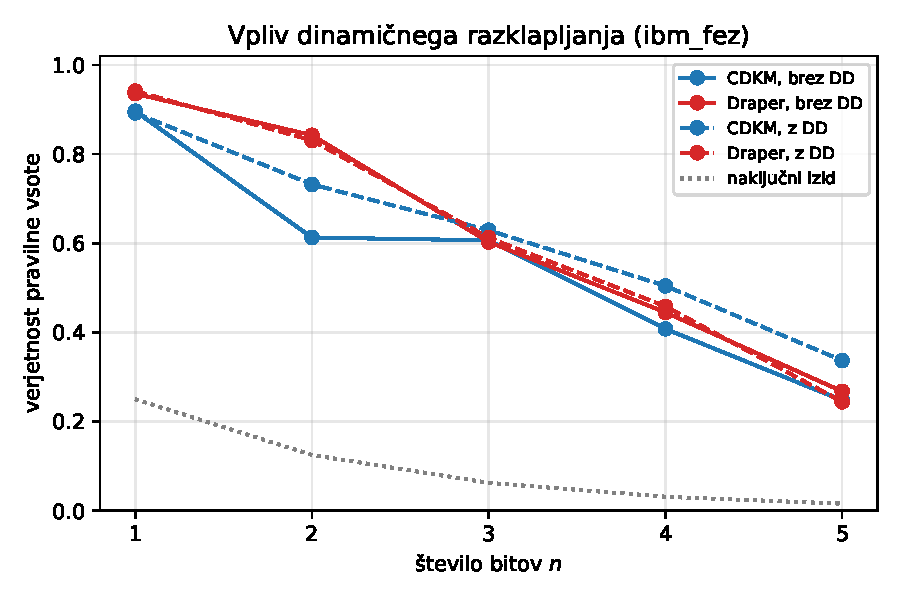
\includegraphics[width=\textwidth]{dd_fez}
\caption{ibm\_fez, $n = 1$ do $5$}
\label{g08:fig:dd}
\end{subfigure}
\hfill
\begin{subfigure}[t]{0.49\textwidth}
\centering
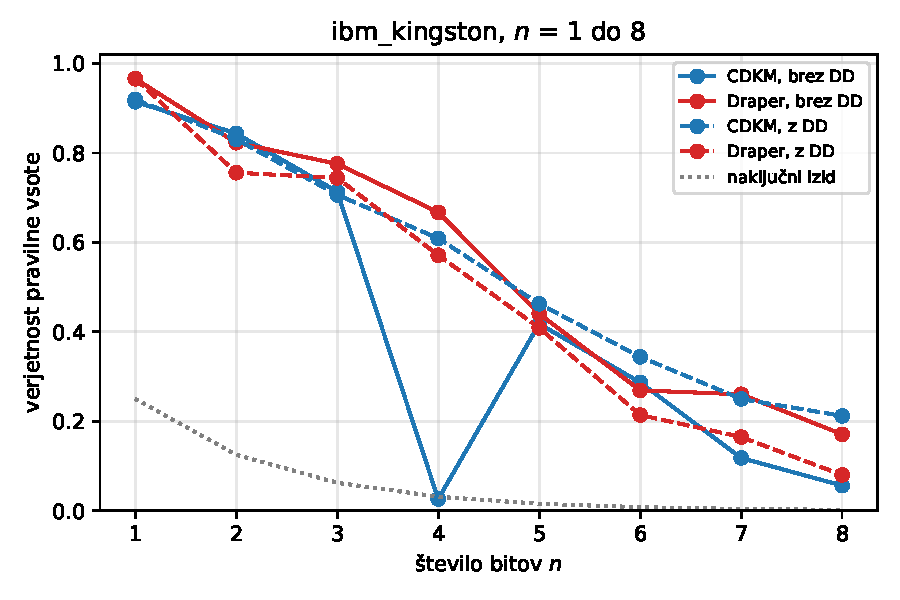
\includegraphics[width=\textwidth]{kingston_n8}
\caption{ibm\_kingston, $n = 1$ do $8$}
\label{g08:fig:kingston}
\end{subfigure}
\caption{Vpliv dinamičnega razklapljanja (DD) na verjetnost pravilne vsote. Polna črta: brez DD, črtkana: z DD.}
\label{g08:fig:ddoba}
\end{figure}

\subsection{Napoved uspešnosti}
\label{g08:sec:napoved}

Tabela~\ref{g08:tab:korelacija} kaže, kako dobro posamezne količine napovedo uspešnost vezij. Vse so močno povezane z uspešnostjo, saj se vse spreminjajo z $n$. Čas izvajanja, ki upošteva tudi mirovanje, je v vseh opravilih boljši napovedovalec od števila dvokubitnih vrat in od ESP. Izmerjene vrednosti so pod napovedjo ESP, a ne enako za oba seštevalnika (slika~\ref{g08:fig:esp}): brez DD je CDKM pri $n \ge 2$ dosegel 50 do 58~\% napovedi ESP, Draper 71 do 73~\%, z DD pa oba približno enak delež (63 do 72~\%). CDKM ima torej brez DD vir napak, ki ga ESP ne zajame in ki ga DD odpravi.

\begin{table}[tbp]
\caption{Pearsonov korelacijski koeficient med izmerjeno verjetnostjo pravilne vsote in napovedovalci na vseh vezjih opravila. V oklepaju je vrednost brez 16 vezij CDKM pri $n = 4$ (razdelek~\ref{g08:sec:neuspehi}).}
\label{g08:tab:korelacija}
\centering
\small
\begin{tabular}{lcccc}
\toprule
Opravilo & ESP & 2q po prev. & Globina & Čas izvajanja \\
\midrule
ibm\_fez brez DD & $+0{,}86$ & $-0{,}85$ & $-0{,}95$ & $-0{,}94$ \\
ibm\_fez ponovitev & $+0{,}87$ & $-0{,}86$ & $-0{,}96$ & $-0{,}95$ \\
ibm\_fez z DD & $+0{,}97$ & $-0{,}95$ & $-0{,}94$ & $-0{,}99$ \\
ibm\_kingston brez DD & $+0{,}68$ ($+0{,}81$) & $-0{,}61$ & $-0{,}83$ & $-0{,}80$ \\
ibm\_kingston z DD & $+0{,}94$ & $-0{,}88$ & $-0{,}96$ & $-0{,}98$ \\
\bottomrule
\end{tabular}
\end{table}

\begin{figure}[tbp]
\centering
\begin{subfigure}[t]{0.40\textwidth}
\centering
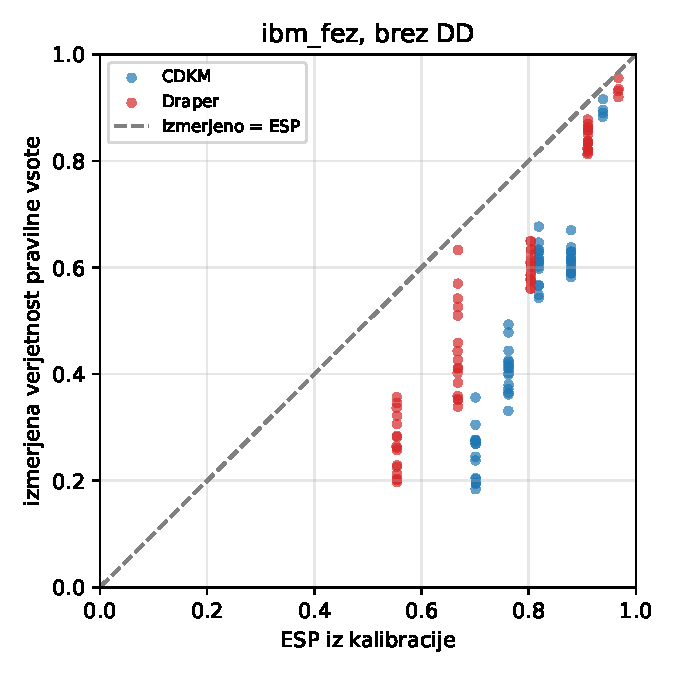
\includegraphics[width=\textwidth]{esp_brez_dd}
\caption{brez DD (ponovitev)}
\end{subfigure}
\hfill
\begin{subfigure}[t]{0.40\textwidth}
\centering
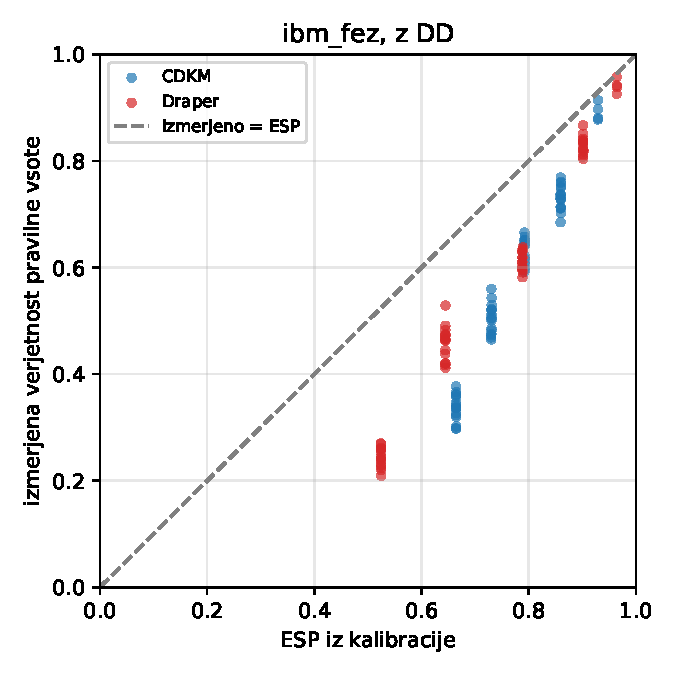
\includegraphics[width=\textwidth]{esp_dd}
\caption{z DD}
\end{subfigure}
\caption{Izmerjena verjetnost pravilne vsote v odvisnosti od ESP za vsa vezja na ibm\_fez. Črtkana črta označuje ujemanje z napovedjo.}
\label{g08:fig:esp}
\end{figure}

Pri $n \ge 4$, kjer ima CDKM jasno manj vrat, je napoved brez DD veljala le v 1 od 9 primerjav (štiri na ibm\_fez in pet na ibm\_kingston), z DD pa v vseh 7 (dve na ibm\_fez in pet na ibm\_kingston). Pri $n \le 2$, kjer ima manj vrat Draper, je napoved veljala na ibm\_fez, na ibm\_kingston pa je bil pri $n = 2$ obakrat boljši CDKM. ESP napove zmagovalca enako kot število vrat, saj je pri vseh $n \ge 3$ višja za CDKM.


\section{Razprava}
\label{g08:sec:razprava}

\smallskip\noindent\textbf{Odgovor na raziskovalno vprašanje.} Kateri seštevalnik je boljši, je odvisno od DD. Brez DD je Draper boljši ali enako dober pri večini $n$, z DD pa je CDKM boljši od $n = 3$ oziroma $4$ naprej, pri $n = 8$ 2,6-krat. Število dvokubitnih vrat po prevajanju je boljši seštevalnik napovedalo le z DD, zato hipoteze ne moreva potrditi. Ne drži niti njena predpostavka, saj ima CDKM pri $n = 2$ več dvokubitnih vrat kot Draper, pri $n = 3$ pa enako.

\smallskip\noindent\textbf{Zakaj DD pomaga seštevalniku CDKM.} Pri CDKM se prenos računa zaporedno, zato veliko kubitov dolgo čaka: pri $n = 5$ na ibm\_fez je skupni čas mirovanja kubitov pri CDKM 83~\si{\micro\second}, pri Draperju 69~\si{\micro\second}. Med mirovanjem kubiti izgubljajo koherenco, zaradi stalne sklopitve ZZ s sosednjimi kubiti pa se kopičijo tudi koherentne fazne napake~\cite{g08:tripathi2022}. Teh napak ESP in število vrat ne zajameta, DD pa jih zaduši~\cite{g08:ezzell2023}. To se ujema z razmerjem med izmerjeno uspešnostjo in ESP (razdelek~\ref{g08:sec:napoved}). Pri Draperju so kubiti bolj enakomerno zaposleni, zato DD odpravi manj napak, dodatni impulzi pa jih lahko celo dodajo, kar bi pojasnilo poslabšanje na ibm\_kingston. Natančnega mehanizma z najinimi meritvami ne moreva določiti.

\smallskip\noindent\textbf{Primerjava z literaturo in s klasično rešitvijo.} Ugotovitev Nishia in sod.~\cite{g08:nishio2020}, da je ocena iz napak vrat uporabno, a nepopolno vodilo, velja tudi za najina procesorja brez DD. Z DD je ESP zelo dober napovedovalec ($r = 0{,}94$ do $0{,}97$). Basili in sod.~\cite{g08:basili2025} so pokazali, da lahko seštevalnik QFT ob šumu izboljšamo z aproksimativno QFT, ki izpusti vrata z majhnimi koti; tega nisva preizkusila, zato je najin Draper verjetno slabši, kot bi lahko bil. Klasični seštevalnik z zaporednim prenosom potrebuje $n$ polnih seštevalnikov s po petimi logičnimi vrati in je praktično vedno pravilen, CDKM kot njegova reverzibilna različica pa pri $n = 5$ potrebuje 124 dvokubitnih vrat in vrne pravilno vsoto v četrtini do polovici ponovitev. Kvantni seštevalnik je zato smiseln le kot del večjega algoritma, ki sešteva superpozicije števil~\cite{g08:vedral1996}.

\smallskip\noindent\textbf{Omejitve.} Uporabila sva dva procesorja iste vrste (Heron r2) in vsak poskus izvedla enkrat ali dvakrat v eni uri, zato so razlike pod približno 0,03 v okviru razlik med zagoni. Pri $n \ge 3$ sva preizkusila le 16 od $4^n$ parov vhodov. Blaženje napak pri meritvah, aproksimativna QFT ali prevajanje, ki upošteva napake posameznih kubitov, bi lahko razmerje med seštevalnikoma spremenili.

\subsection{Kaj ni delovalo}
\label{g08:sec:neuspehi}

\smallskip\noindent\textbf{Izstopajoč rezultat na ibm\_kingston.} Pri opravilu brez DD je CDKM pri $n = 4$ vrnil pravilno vsoto le v 2,6~\% ponovitev, kar je manj od naključnega izida (3,1~\%). V vseh 16 vezjih je bil v 84 do 93~\% ponovitev napačen isti bit vsote, $s_3$, izmerjen na fizičnem kubitu 79. Kalibracija za ta kubit ne kaže ničesar posebnega (napaka meritve 0,7~\%, $T_1 = 274$~\si{\micro\second}), ESP pa napove uspešnost 0,81. Opravilo z DD dve minuti pozneje je na istih kubitih doseglo 0,61. Ker je bit obrnjen skoraj vedno in ne naključno, gre verjetno za koherentno napako med mirovanjem, ki jo DD odpravi. Rezultata pri primerjavi seštevalnikov zato ne upoštevava.

\smallskip\noindent\textbf{Šumni simulator ni napovedal izidov na procesorju.} Po šumnem simulatorju bi moral biti CDKM pri $n = 5$ pravilen v 69~\% ponovitev, na procesorju brez DD pa je bil v 27~\% in ni bil boljši od Draperja. Model v Qiskit Aer upošteva napake vrat in meritev iz posnetka kalibracije, ne pa, kolikor nama je znano, presluha med kubiti in napak med mirovanjem, ki so pri CDKM pomembne.

\smallskip\noindent\textbf{Neprimerljiva metrika pred prevajanjem.} Sprva sva primerjala število dvokubitnih vrat pred prevajanjem in dobila napačen vtis, da ima CDKM veliko manj vrat (pri $n = 5$ 21 proti 50), ker to število ne zajame trokubitnih Toffolijevih vrat. Po razgradnji na vrata CNOT ima pri $n \le 3$ manj vrat Draper.


\section{Zaključek}
\label{g08:sec:zakljucek}

Seštevalnik CDKM ima po prevajanju za procesor IBM Heron od $n = 4$ naprej manj dvokubitnih vrat kot Draperjev seštevalnik, pri $n = 8$ 2,4-krat manj. Na procesorju se ta prednost pokaže le, če uporabimo dinamično razklapljanje: z njim je CDKM boljši pri vseh $n \ge 4$, brez njega pa je Draper boljši ali enako dober pri večini $n$. Število dvokubitnih vrat je zato dober napovedovalec le, kadar so zadušene napake med mirovanjem kubitov, ki jih zaporedni prenos pri CDKM poveča. Delo bi lahko nadaljevali s ponovitvami poskusov ob različnih urah, z aproksimativno QFT pri Draperju, z blaženjem napak pri meritvah in s seštevalnikom z vnaprejšnjim izračunom prenosa, ki ima logaritmično globino~\cite{g08:draper2006}.


\section*{Doprinosi avtorjev}

Jurij Anžič je implementiral in testiral seštevalnik CDKM, napisal skupni del kode za pripravo vezij, prevajanje, metrike in zagon na simulatorjih ter test dogovora o vmesniku. Pripravil je osnutek poročila.

Janez Koprivec je pripravil prijavo teme in razvojno okolje ter implementiral in testiral Draperjev seštevalnik. Napisal je kodo za zagon na procesorjih IBM in analizo opravil ter izvedel poskuse na procesorjih IBM.

Oba sta sodelovala pri interpretaciji rezultatov.

\section*{Izjava o uporabi generativne umetne inteligence}

Pri delu sva uporabljala jezikovni model Claude (Anthropic). Pomagal je pri pisanju in pregledu kode (seštevalnik CDKM, skupni del in testi), pri iskanju vzroka za izstopajoč rezultat na ibm\_kingston, pri iskanju virov in pri pisanju osnutka poročila. Vse rezultate sva preverila s testi in ponovnim izvajanjem, vire sva preverila, besedilo pa pregledala in popravila.
